% =============================================================================================================
% Environmental Research Letters (IOP Publishing) -- Letter manuscript, Phase 1 / Stage B only
% Compile: pdflatex main && bibtex main && pdflatex main && pdflatex main
% Uses the IOP class `iopart` (+ iopart-num.bst) when it is installed (e.g. on Overleaf with the IOP template);
% otherwise falls back to a plain `article` layout with the same macros so that the manuscript compiles anywhere.
% Every number in Sections 2-5 is checked against DELIVERABLES_DAMARAKUNTA_STAGE_B by paper/erl/verify_erl_numbers.py.
% =============================================================================================================
\IfFileExists{iopart.cls}{%
  \documentclass[12pt]{iopart}\newcommand{\ERLiop}{}\newcommand{\ERLbst}{iopart-num}}{%
  \documentclass[12pt,a4paper]{article}\newcommand{\ERLbst}{unsrt}}
\usepackage{graphicx}
\usepackage{booktabs}
\usepackage{array}
\usepackage{amsmath,amssymb}
\usepackage[hidelinks]{hyperref}
\setlength{\emergencystretch}{3em}
\providecommand{\ERLiop}{\relax}
\makeatletter
\@ifclassloaded{iopart}{}{%
  \usepackage[margin=2.5cm]{geometry}\usepackage{setspace}\onehalfspacing
  \newcommand{\address}[1]{\gdef\ERL@address{#1}}
  \newcommand{\ead}[1]{}
  \newcommand{\submitto}[1]{}
  \newcommand{\ack}{\section*{Acknowledgments}}
  \usepackage{environ}\newcommand{\ERL@kw}{}\newcommand{\ERL@abs}{}
  \RenewEnviron{abstract}{\xdef\ERL@abs{\unexpanded\expandafter{\BODY}}}
  \newcommand{\ERLkeywords}[1]{\gdef\ERL@kw{#1}}
  \renewcommand{\title}[2][]{\gdef\ERL@title{#2}}
  \renewcommand{\author}[1]{\gdef\ERL@author{#1}}
  \renewcommand{\maketitle}{\begin{center}{\Large\bfseries\ERL@title\par}\vspace{0.8em}{\large\ERL@author\par}\vspace{0.4em}{\small\ERL@address\par}\end{center}\vspace{0.5em}\begin{quote}\small\textbf{Abstract.} \ERL@abs\end{quote}\vspace{0.4em}\noindent{\small\textit{Keywords}: \ERL@kw}\par\bigskip}
}
\@ifclassloaded{iopart}{\newcommand{\ERLkeywords}[1]{\noindent{\it Keywords\/}: #1\par}}{}
\makeatother
\newcommand{\dinoseg}{StrongDINOv2Seg}
\newcommand{\Lcost}{L_{\mathrm{cost}}}

\begin{document}

\title[Missed buildings and shared rural access roads]{Missed buildings and shared rural access roads: propagating satellite building-detection omissions through road planning in a Telangana village, India}

\author{Pendyala Archana}
\address{Chaitanya Bharathi Institute of Technology (CBIT), Hyderabad, Telangana, India}
% TODO (author): add supervisor / co-author name, designation, department and corresponding-author e-mail (\ead{...}).
\submitto{\ERL}

\begin{abstract}
Extending all-weather road access to dispersed rural hamlets is a major source of new linear infrastructure, yet planning still relies on manually digitised building inventories, and automated detectors are judged by pixel overlap rather than by the plans they feed. We couple a fine-tuned DINOv2 segmenter (StrongDINOv2Seg; 53.8\% mIoU on the LoveDA validation split) and an instance-extraction step with a 10~m cost surface (land cover, slope, building-footprint penalty) and a shared-network planner for Damarakunta village, Siddipet district, Telangana, India (18.5~km$^2$). The shared plan connects 163 houses and five facilities; the house network needs 5{,}069~m of new corridor, 24.9\% less unique length than independent house-by-house routes (6{,}753~m). Because corridors are shared, this saving is stable (24.9--26.6\%) under simulated detection errors, but the plan itself is not: omitting 10--20\% of buildings at random shortens the corridor by 7.6--16.9\% and leaves 16--33 households without a planned route, and omitting the 62 merged-roof blobs shortens it by 29.4\% and leaves 38.0\% of households unserved. Total corridor length alone therefore understates road need when detections are incomplete. We recommend reporting instance-level recall and unserved households alongside IoU. Results are model outputs for one village without field validation.
\end{abstract}

\ERLkeywords{rural roads, building footprint extraction, satellite remote sensing, least-cost path, shared network, error propagation, land take, Telangana}

\maketitle

\section{Introduction}
Road building is among the most consequential land-use changes of the coming decades. Global road length is projected to grow by roughly 3.0--4.7 million km by 2050 \cite{meijer2018global}, and new roads open land to clearing, fragmentation and conversion \cite{laurance2014global}. Much of this growth is local. In India the Pradhan Mantri Gram Sadak Yojana (PMGSY) connects unconnected habitations by all-weather roads \cite{pmgsy}, and each connection cuts a corridor through farmland and village commons. Where a corridor runs, and how many separate corridors are built, are planning decisions that can be improved before any land is taken.

Planning access to individual hamlets needs three inputs: where the dwellings are, what land a corridor must cross, and a rule that turns these into alignments. In practice dwellings are digitised by hand, which is slow and subjective, and each house is often treated as its own connection problem, so neighbouring houses re-trace the same corridor. Deep learning now maps buildings at continental scale \cite{ji2019whu,sirko2021openbuildings}, and vision foundation models promise better transfer to scenes with few labels \cite{oquab2023dinov2,cong2022satmae}. But detectors are scored by pixel overlap (IoU, Dice), whereas a planner consumes \emph{instances}: a missed house is a household without a connection, a smaller corridor budget, and possibly a corridor through a roof the planner did not know about. How detection errors propagate through such a planning graph is rarely measured, although the general problem of error propagation in spatial analysis is well known \cite{heuvelink1998error,foody2002status}.

We close this loop for one village. We build a pipeline from satellite imagery to a shared access network, and use controlled omission and addition scenarios to ask three questions. (i) How much unique corridor length does sharing save over house-by-house routing? (ii) How does a soft penalty on building footprints trade corridor length against the number of dwellings a route crosses? (iii) How do missed (or spurious) buildings change planned length, household coverage and exposure? The study is a single-village case study without field validation; its outputs are planning alternatives, not engineered alignments.

\section{Study area and data}
\subsection{Damarakunta}
Damarakunta is a rural revenue village in Markook mandal, Siddipet district, Telangana ($\approx 17.707^{\circ}$N, $78.753^{\circ}$E). Its administrative boundary, from the Telangana State Remote Sensing Application Centre (TGRAC), encloses 18.47~km$^2$ (UTM zone 44N, EPSG:32644; figure~\ref{fig:area}). Settlement is dispersed: houses form small clusters separated by agricultural land. TGRAC records four facilities (two schools, a health sub-centre and an anganwadi). The anganwadi was excluded because its coordinate lies 371~m from the nearest detected footprint and 126~m from the nearest independent building polygon; two Gram Panchayat headquarters points were added as administrative utilities, giving five facilities. The TGRAC road layer has 43 features totalling 93.5~km, of which 51.7~km remain after clipping to the boundary (44.7\% of the original length lies outside it).

\begin{figure}[t]
\centering
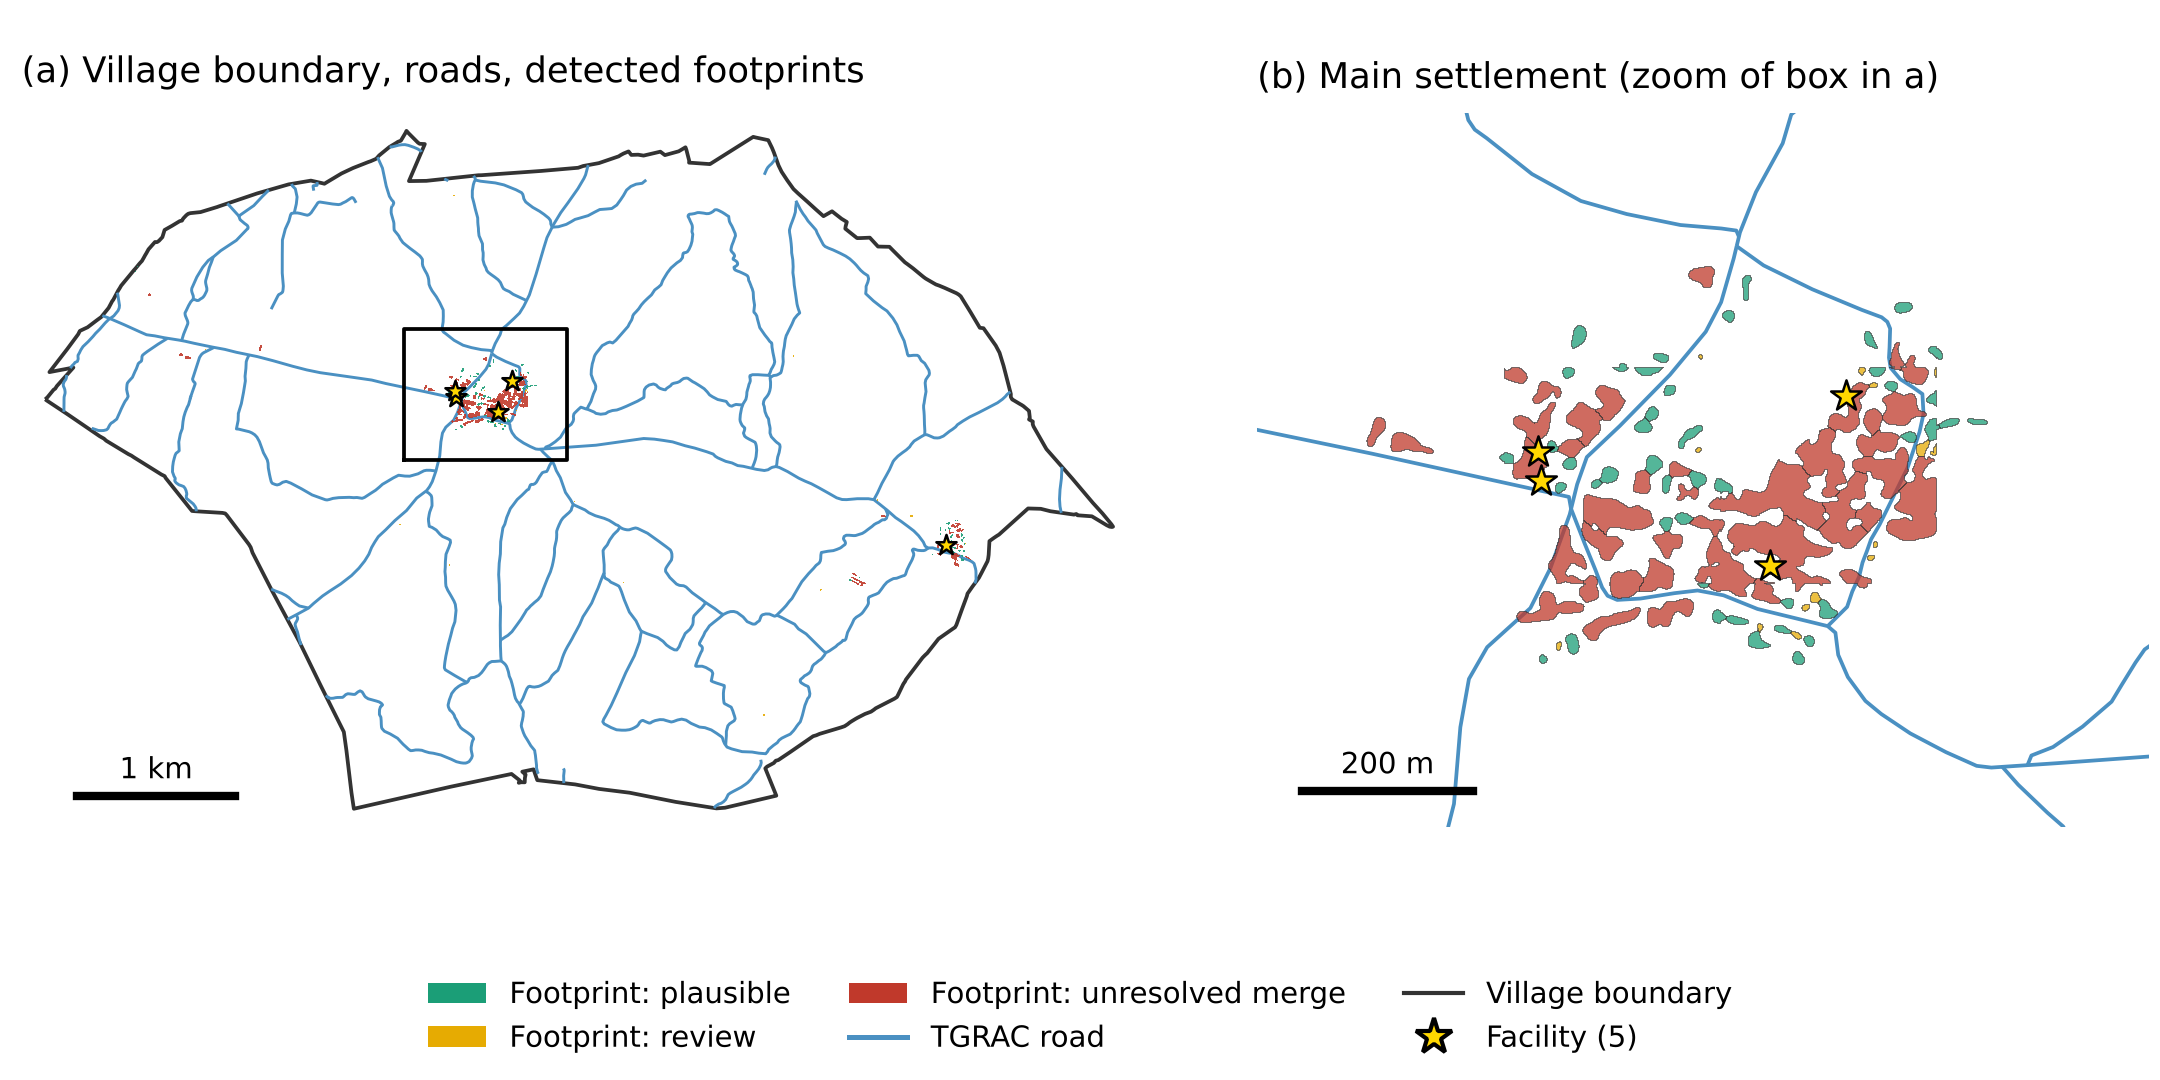
\includegraphics[width=\textwidth]{figures/fig2_study_area.png}
\caption{Study area. (a)~Damarakunta boundary, TGRAC roads and detected building footprints coloured by quality class, with the five facilities. (b)~Main settlement (box in a). Footprints are automatic detections, not a census. No imagery basemap is shown because the imagery licence for derived products is unresolved.}
\label{fig:area}
\end{figure}

\subsection{Data}
Table~\ref{tab:data} lists the inputs. A 0.6~m, three-band mosaic (11{,}296 $\times$ 7{,}171 px) was assembled from Esri World Imagery map exports; its capture date was recorded at one sampled point only (29 April 2026). Slope is computed with a Sobel operator from a $\sim$30~m DEM (the file name indicates an SRTM 1~arc-second tile; its source was not recorded) and bilinearly resampled to 10~m, so it carries no true 10~m terrain detail. ESA WorldCover supplies land cover at 10~m \cite{zanaga2021worldcover}. All layers are aligned to a 432 $\times$ 679 cell grid at 10~m. Cells that are water, no-data or steeper than 25$^{\circ}$ are blocked; 961 slope cells and 178 land-cover cells without data are treated as invalid, not interpolated.

\begin{table}[t]
\caption{Input data. ``Status'' records what is known about licensing; none of the layers was verified against ground truth.}
\label{tab:data}
\centering
\small
\begin{tabular}{@{}p{3.2cm}p{5.6cm}p{5.2cm}@{}}
\toprule
Layer & Source and resolution & Status \\
\midrule
Village boundary, roads, facilities & TGRAC web services (43 road features) & Licence not stated; road completeness unverified \\
Imagery & Esri World Imagery export, 0.6~m, 3 bands & Licence for derived products unresolved; not redistributed \\
Land cover & ESA WorldCover v200 (2021), 10~m \cite{zanaga2021worldcover} & CC BY 4.0 \\
Terrain & $\sim$30~m DEM, Sobel slope & Source not recorded \\
Reference footprints (proxy) & Google Open Buildings v3 \cite{sirko2021openbuildings}, 1{,}537 polygons in the boundary & CC BY 4.0 / ODbL; used only for a proxy agreement check \\
Training benchmark & LoveDA \cite{wang2021loveda} & Source domain only \\
\bottomrule
\end{tabular}
\end{table}

\subsection{Building candidates and evaluation without ground truth}
Building candidates are model outputs: 278 polygons, 165 inside the boundary, of which 163 are retained as routing targets. They carry a quality class: \textsc{Plausible} (71), \textsc{Review} (32) and \textsc{Unresolved\_Merge} (62), the last denoting blobs that merge several adjacent roofs and could not be split. No pixel-level reference exists for Damarakunta, so two evaluations are kept distinct: source-domain validation of the segmenter on LoveDA, and a \emph{proxy agreement} check of the village candidates against Open Buildings v3 (a candidate agrees if an Open Buildings polygon lies within 30~m). Agreement is not accuracy, and neither layer is treated as truth.

\section{Methods}
\subsection{Building and facility extraction}
Figure~\ref{fig:workflow} summarises the workflow. \dinoseg{} is a fully fine-tuned DINOv2 ViT-B/14 encoder \cite{oquab2023dinov2}. Tokens from blocks 3, 6, 9 and 12 are projected to 256 channels, fused (FPN-style \cite{lin2017fpn}) and passed through an ASPP neck \cite{chen2018deeplabv3plus} and a four-stage residual decoder with auxiliary heads for deep supervision \cite{lee2015dsn}. The loss combines cross-entropy, soft Dice \cite{milletari2016vnet} and a Sobel-weighted boundary term with weights $(0.5, 0.4, 0.1)$. Training used AdamW, cosine annealing over 10 epochs and the eight-class LoveDA convention with class 0 ignored; the epoch-4 checkpoint, best on validation, was applied to the mosaic in $560\times560$~px tiles (stride 420~px). The class map was converted to instances with a distance-transform procedure (OpenCV and NumPy): adjacent pieces are separated only where the saddle between them is narrower than 0.65 times the inscribed radius of the smaller piece, polygons much larger than a typical roof are flagged \textsc{Unresolved\_Merge} rather than cut, and the remainder is classed \textsc{Plausible} or \textsc{Review} by shape, probability and isolation flags. The representative point of each polygon becomes a routing target with weight one; facility points form a second target set.

\subsection{Cost surface}
Let $\mathcal{B}$ be blocked cells (water, no-data, slope $>25^{\circ}$) and $\mathcal{P}$ the cells intersecting a candidate footprint. The planning graph has the unblocked cells as nodes and 8-neighbour edges with no diagonal corner-cutting. The cost of a cell is
\begin{equation}
c(x)=\bigl[c_{\mathrm{lc}}(\ell(x))+g(s(x))\bigr]\,m(x),\qquad m(x)=\begin{cases}\mu & x\in\mathcal{P}\\ 1 & \text{otherwise,}\end{cases}
\label{eq:cell}
\end{equation}
where $\ell$ is the land-cover class, $c_{\mathrm{lc}}$ a tabulated resistance, $g$ a non-decreasing slope term and $\mu=4$ the footprint penalty. Edge weights are the mean end-cell cost times step length. Costs are ordinal planning units, not currency. Around the health sub-centre, whose point lies on the edge of its own footprint, the penalty is lifted within a 20~m disc so that the route is not forced to detour around its own building. Crossing statistics are always computed on the original footprints.

\subsection{Shared-network planner}
For each target, Stage~A computes a least-cost path to the existing road cells with Dijkstra-type search \cite{dijkstra1959note,hart1968astar,collischonn2000lcp} and up to two further alternatives by inflating costs by factors 3 and 8 in a 20~m corridor around earlier paths (overlap $\le 0.8$; 319 alternatives for 163 houses). Stage~B selects greedily the (target, alternative) pair with the highest weight per \emph{marginal} cost,
\begin{equation}
\Delta\Lcost\bigl(\pi\mid S\bigr)=\sum_{e\in\pi\setminus E_S}w(e),
\label{eq:marginal}
\end{equation}
where $E_S$ is the edge set already selected, so built edges are free and a route may end on another route. This is the shortest-path heuristic for Steiner trees \cite{kou1981steiner,mehlhorn1988steiner,hwang1992steiner} applied to a penalised, land-cover-weighted graph with the road network as a free sub-tree; it carries no optimality guarantee. Two passes of leaf re-routing follow. Facilities are planned before houses. We compare with (i) straight lines, (ii) independent least-cost routes, (iii) a length-only control (shortest distance under the same constraints) and (iv) a roads-only shared reference. With $L(\cdot)$ the unique edge length, the saving is $\rho=100\,(L_{\mathrm{indep}}-L_{\mathrm{plan}})/L_{\mathrm{indep}}$.

\subsection{Omission and addition scenarios}
Let $T$ be the target set and $M\subset T$ an omitted set standing for false negatives. The planner is re-run on $T\setminus M$ with the footprints of $M$ also removed from the penalty layer, because a missed detection is absent from both the target list and the obstacle layer. We report coverage $\kappa=|T\setminus M|/|T|$, unserved households $U=|T|-|\text{routed}|$, the change in unique length $\delta_L=(L(T\setminus M)-L(T))/L(T)$ and length per routed target $\bar{\ell}=L/|\text{routed}|$, which is the comparable quantity because absolute length shrinks mechanically when fewer targets are connected. Scenarios are random omission of 10\% and 20\% of targets (five draws each), omission of the smallest 10\% and 25\% of targets by footprint area, omission of all 62 \textsc{Unresolved\_Merge} candidates, and random additions of 10\% and 20\% synthetic targets as a false-positive analogue. Omission scenarios are synthetic, not measured detection errors.

\begin{figure}[t]
\centering
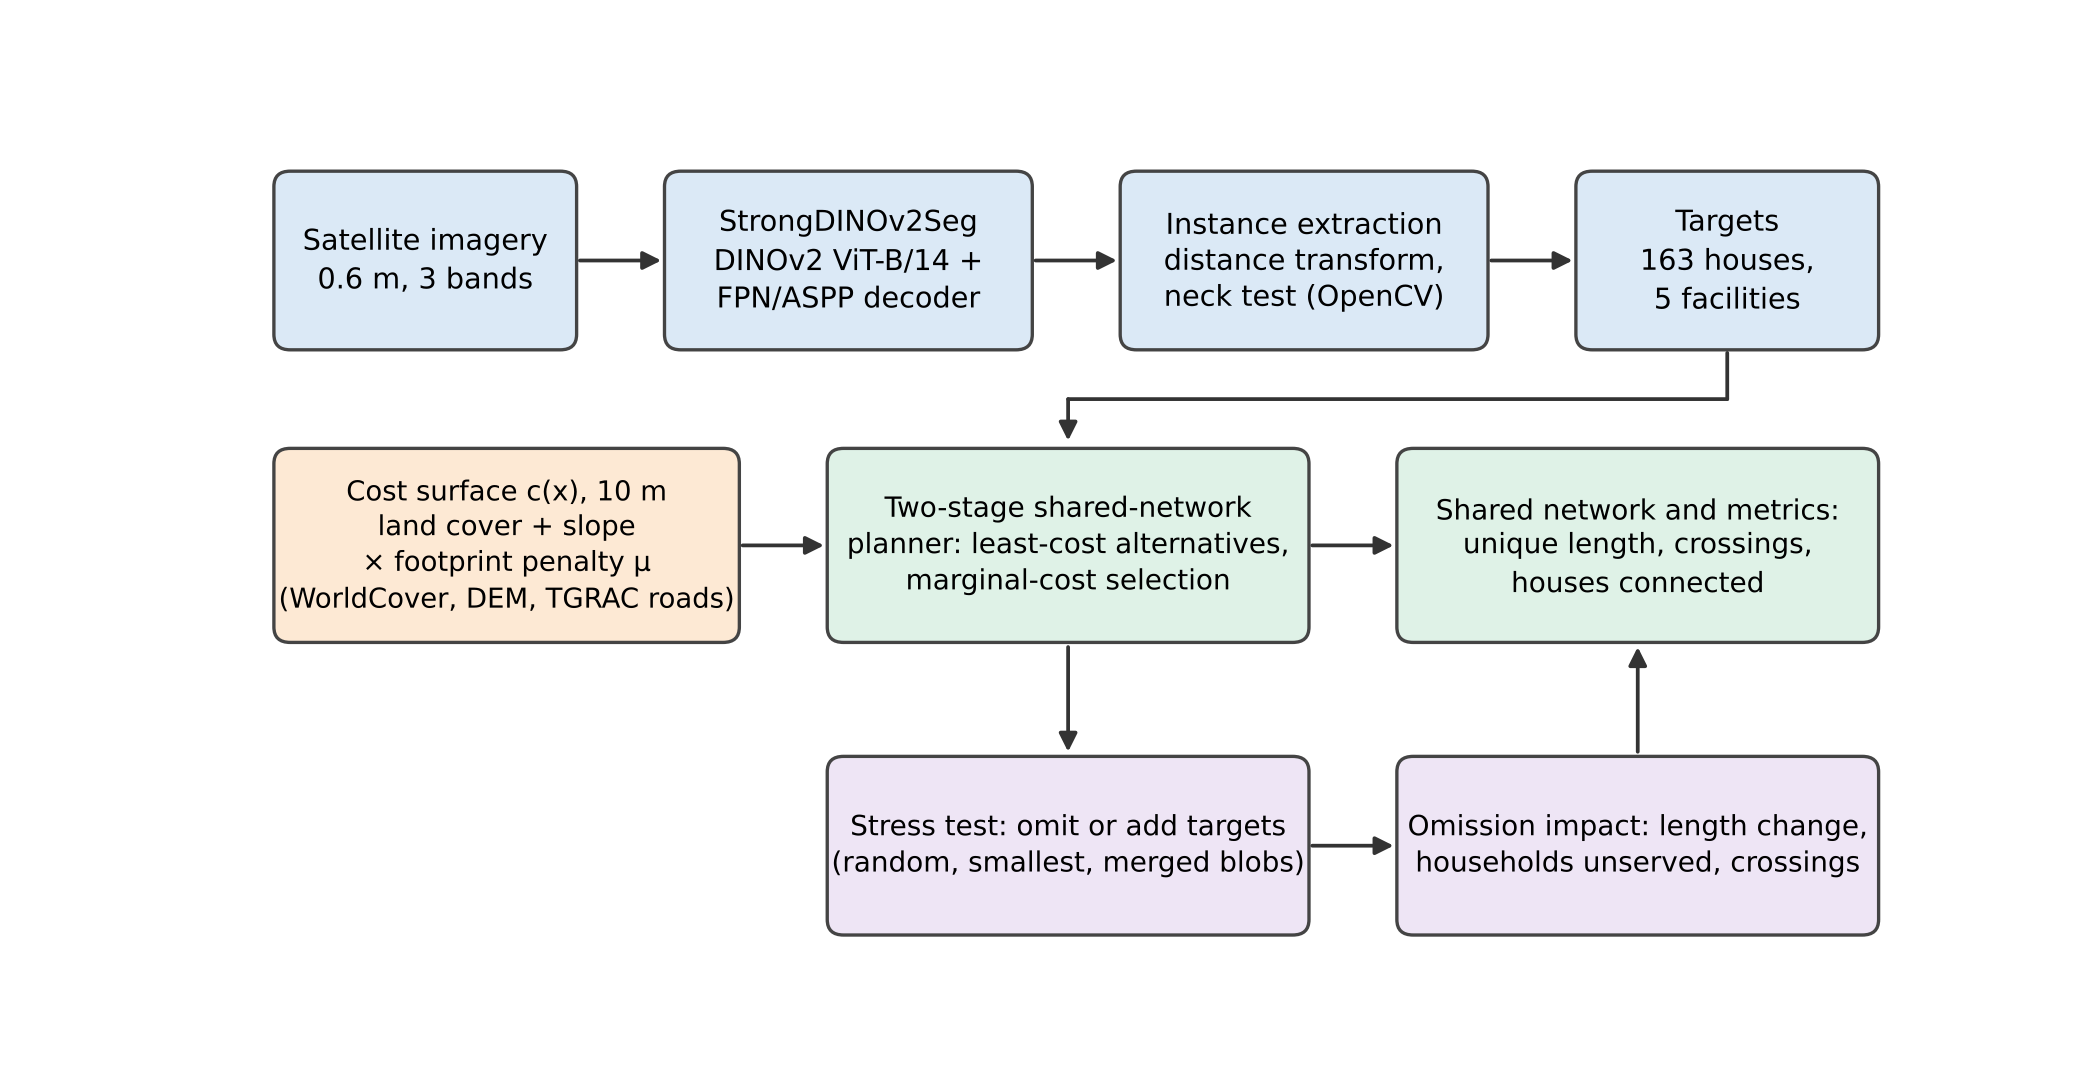
\includegraphics[width=\textwidth]{figures/fig1_workflow.png}
\caption{Workflow. Imagery is segmented by StrongDINOv2Seg and converted to instances; targets and the cost surface feed a two-stage shared-network planner, and controlled omissions and additions are propagated through the planner to measure their effect on length, coverage and exposure.}
\label{fig:workflow}
\end{figure}

\section{Results}
\subsection{Detection}
On the 1{,}669-image LoveDA validation split (560~px, seven scored classes) the epoch-4 checkpoint reached 53.8\% mIoU, 68.9\% Dice and 71.3\% pixel accuracy, with 72.4\% macro precision and 66.9\% macro recall (table~\ref{tab:seg}); these are source-domain figures and not accuracy on Damarakunta. For the Building class IoU is 54.0\%, precision 62.1\% and recall 80.6\%. Of the 165 in-boundary candidates, 118 (71.5\%) agree with Open Buildings; agreement ranges from 43.8\% for \textsc{Review} to 85.5\% for \textsc{Unresolved\_Merge}. High agreement of merged blobs says nothing about whether a blob holds one house or several, which is what matters for per-household routing. Conversely, Open Buildings lists 1{,}537 polygons in the boundary, of which 1{,}186 have no candidate, so the candidate set is not a complete house count; the 163 targets are a conservative planning set.

\begin{table}[t]
\caption{Detection evaluation. Top: LoveDA validation (source domain); precision and recall are macro-averages over the seven scored classes. Bottom: agreement of the 165 Damarakunta candidates with Open Buildings v3 (a proxy, not accuracy).}
\label{tab:seg}
\centering
\small
\begin{tabular}{@{}lrrrrr@{}}
\toprule
\multicolumn{6}{@{}l}{\textit{LoveDA validation split (\%)}}\\
 & mIoU & Dice & Pixel acc. & Precision & Recall\\
\midrule
StrongDINOv2Seg & 53.8 & 68.9 & 71.3 & 72.4 & 66.9\\
\quad Building class & 54.0 & 70.1 & --- & 62.1 & 80.6\\
\midrule
\multicolumn{6}{@{}l}{\textit{Damarakunta candidates vs.\ Open Buildings v3}}\\
Class & Candidates & Agree & Disagree & \multicolumn{2}{c}{Agreement (\%)}\\
\midrule
All & 165 & 118 & 47 & \multicolumn{2}{c}{71.5}\\
\textsc{Plausible} & 71 & 51 & 20 & \multicolumn{2}{c}{71.8}\\
\textsc{Review} & 32 & 14 & 18 & \multicolumn{2}{c}{43.8}\\
\textsc{Unresolved\_Merge} & 62 & 53 & 9 & \multicolumn{2}{c}{85.5}\\
\bottomrule
\end{tabular}
\end{table}

\subsection{Shared network}
Independent least-cost routes for the 163 houses total 10{,}045~m, but because neighbouring houses re-trace the same corridors the unique built length is 6{,}753~m (table~\ref{tab:routing}, figure~\ref{fig:routing}a). The two-stage plan reduces this to 5{,}069~m, a saving of 1{,}684~m (24.9\%). All 163 houses and five facilities are connected (168 of 168 verified by the planner), with no hard-constraint violation, no cycle and no route that crosses another without a shared cell. A length-only control is \emph{longer} in unique length than independent least-cost routing (6{,}980~m, $+3.4$\%) and crosses other footprints on 64 routes, so the cost surface, not shortness alone, produces the gain. The roads-only shared reference (5{,}229~m) is 160~m longer than the two-stage plan, so routes ending on other routes contribute a modest further saving. Extra alternatives change nothing in this village ($K=1$ and $K=3$ give identical lengths) and leaf re-routing contributes 10.3~m (0.2\%), so the saving comes mainly from sharing itself. One house (C0002) attaches to a road fragment that the raster treats as a separate component, which we regard as a boundary-truncation artefact of the clipped domain; on the road lines it connects to the main network.

\begin{table}[t]
\caption{Routing efficiency for 163 houses ($\mu=4$ unless stated). Total length counts every route; unique length counts shared edges once. Crossings count routes through another house's footprint. $\rho$ is the saving in unique length against independent least-cost routes.}
\label{tab:routing}
\centering
\footnotesize
\begin{tabular}{@{}>{\raggedright\arraybackslash}p{4.3cm}rrrrr@{}}
\toprule
Strategy & Total (m) & Unique (m) & $\rho$ (\%) & Routes crossing & In footprints (m)\\
\midrule
Straight line (2 targets infeasible) & 8{,}092.3 & --- & --- & 60 & 1{,}453.2\\
Independent least-cost routes & 10{,}045.4 & 6{,}753.1 & 0.0 & 46 & 328.3\\
Length-only control & 9{,}166.3 & 6{,}979.8 & $-3.4$ & 64 & 1{,}615.8\\
Roads-only shared reference & 5{,}229.3 & 5{,}229.3 & 22.6 & 29 & 216.1\\
\textbf{Two-stage plan (proposed)} & \textbf{5{,}069.0} & \textbf{5{,}069.0} & \textbf{24.9} & \textbf{28} & \textbf{209.1}\\
\midrule
\multicolumn{6}{@{}l}{\textit{No footprint penalty ($\mu=1$)}}\\
Independent least-cost routes & 9{,}595.9 & 6{,}921.3 & 0.0 & 63 & 1{,}423.1\\
Two-stage plan & 4{,}705.5 & 4{,}705.4 & 32.0 & 56 & 660.1\\
\midrule
\multicolumn{6}{@{}l}{\textit{Buffered footprints (7.1~m), two-stage plan}}\\
Penalty $\mu=20$ & --- & 6{,}238.1 & 18.5 & 19 & 147.9\\
Penalty $\mu=100$ & --- & 6{,}190.3 & 18.9 & 19 & 144.8\\
\bottomrule
\end{tabular}
\end{table}

\begin{figure}[t]
\centering
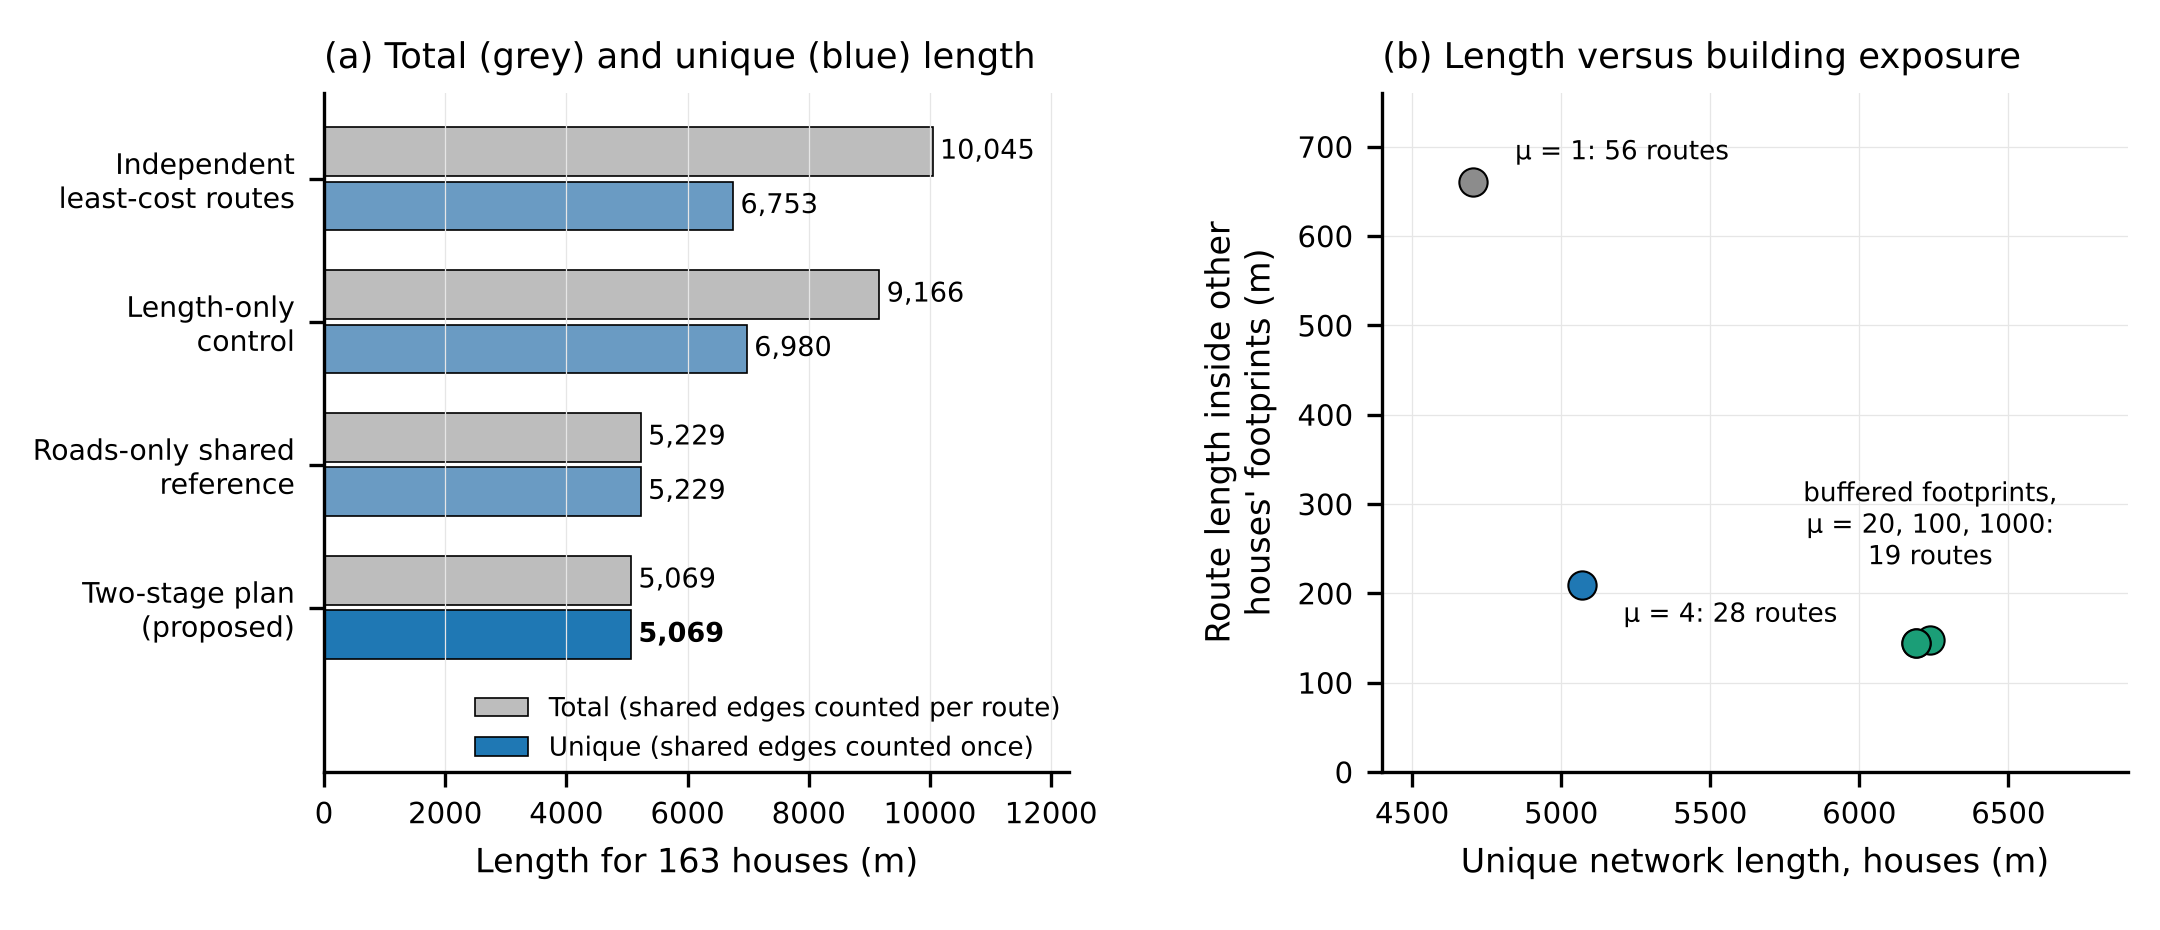
\includegraphics[width=\textwidth]{figures/fig3_routing.png}
\caption{Routing results for 163 houses. (a)~Total and unique corridor length by strategy. (b)~Unique network length against route length inside other houses' footprints for no penalty ($\mu=1$), the primary penalty ($\mu=4$) and buffered footprints with large penalties ($\mu=20$, 100, 1000; the last two coincide).}
\label{fig:routing}
\end{figure}

\subsection{Footprint penalty and the local override}
The footprint penalty exposes a trade-off between corridor length and exposure of dwellings (figure~\ref{fig:routing}b). Without a penalty the plan is shortest (4{,}705~m) but 56 routes pass through other houses (660~m inside footprints). With $\mu=4$ the plan is 364~m (7.7\%) longer, while crossings halve to 28 routes and 209~m. Buffering footprints by 7.1~m with penalties of 20--1000 lowers crossings to 19 routes (145--148~m) but adds 1.1--1.2~km of corridor and erodes the saving to 18.5--19.2\%; the effect saturates by $\mu=20$. Hard blocking was infeasible because every house point lies inside its own blocked cell, and the remaining crossings under buffering are mostly confined to the first 20~m, where a route leaves its own cluster of touching buildings (16 of 19 routes). The health sub-centre point lies 1.8~m from a 1{,}194~m$^2$ unresolved-merge footprint; with the 20~m override its route is 67.4~m long and costs 260.1 units, against 357.7 units without it ($-27.3$\%; recorded in the project notes, not in a result table), and no other house route changes. The override is a manual modelling decision, not a finding about access.

\subsection{Impact of building omissions}
Table~\ref{tab:omission} and figure~\ref{fig:omission} summarise the omission analysis against the 5{,}069~m baseline.

\emph{The plan becomes shorter, not longer.} Missing buildings make the corridor budget look smaller: 10\% random omission (16 houses) understates length by 7.6\%, 20\% by 16.9\%, omission of the smallest quarter by 25.1\% and omission of all merged blobs by 29.4\%. A planner reading only total length would underfund the scheme.

\emph{The vanished households are the ones that lose access.} $U$ households receive no route: 16 and 33 for random 10\% and 20\% omission, 41 for the smallest quarter and 62 (38.0\%) for merged blobs. Merged blobs correspond to dense multi-roof structures; whether they coincide with the dense core of a hamlet was not measured, so concentration of loss is a risk, not a result.

\emph{Length per routed target hides the problem.} It is stable under random omission (31.9~m and 32.4~m against 31.1~m) but rises 14\% when merged blobs are removed (35.4~m), because the remaining targets are peripheral. Random additions lengthen the plan by 8.6\% and 15.8\% but lower the per-target length, since dense additions share existing corridors. The saving $\rho$ against independent routing stays between 24.9\% and 26.6\% in every scenario, so the benefit of sharing is robust even though absolute length is not. These scenarios indicate direction and magnitude, not effect sizes with uncertainty: the merged-blob, smallest-10\% and smallest-25\% scenarios are single deterministic runs, and the random scenarios use five draws.

\begin{table}[t]
\caption{Impact of simulated omissions and additions on the shared network. Baseline: 5{,}069.0~m, 163 routed. Random scenarios are means of five draws. $U$: households without a route; $\kappa$: coverage; $\delta_L$: change in unique length; $\bar\ell$: length per routed target; $\rho$: saving against independent routing.}
\label{tab:omission}
\centering
\small
\begin{tabular}{@{}lrrrrrrr@{}}
\toprule
Scenario & Routed & $U$ & $\kappa$ (\%) & $L$ (m) & $\delta_L$ (\%) & $\bar\ell$ (m) & $\rho$ (\%)\\
\midrule
Baseline & 163 & 0 & 100.0 & 5{,}069.0 & 0.0 & 31.1 & 24.9\\
Omit 10\% (random) & 147.0 & 16 & 90.2 & 4{,}684.4 & $-7.6$ & 31.9 & 25.1\\
Omit 20\% (random) & 130.0 & 33 & 79.8 & 4{,}211.5 & $-16.9$ & 32.4 & 25.0\\
Omit smallest 10\% & 146 & 17 & 89.6 & 4{,}648.7 & $-8.3$ & 31.8 & 24.9\\
Omit smallest 25\% & 122 & 41 & 74.8 & 3{,}798.3 & $-25.1$ & 31.1 & 25.6\\
Omit merged blobs & 101 & 62 & 62.0 & 3{,}579.0 & $-29.4$ & 35.4 & 26.6\\
\midrule
Add 10\% (random) & 177.4 & --- & --- & 5{,}502.4 & $+8.6$ & 31.0 & 25.6\\
Add 20\% (random) & 190.6 & --- & --- & 5{,}868.3 & $+15.8$ & 30.8 & 25.4\\
\bottomrule
\end{tabular}
\end{table}

\begin{figure}[t]
\centering
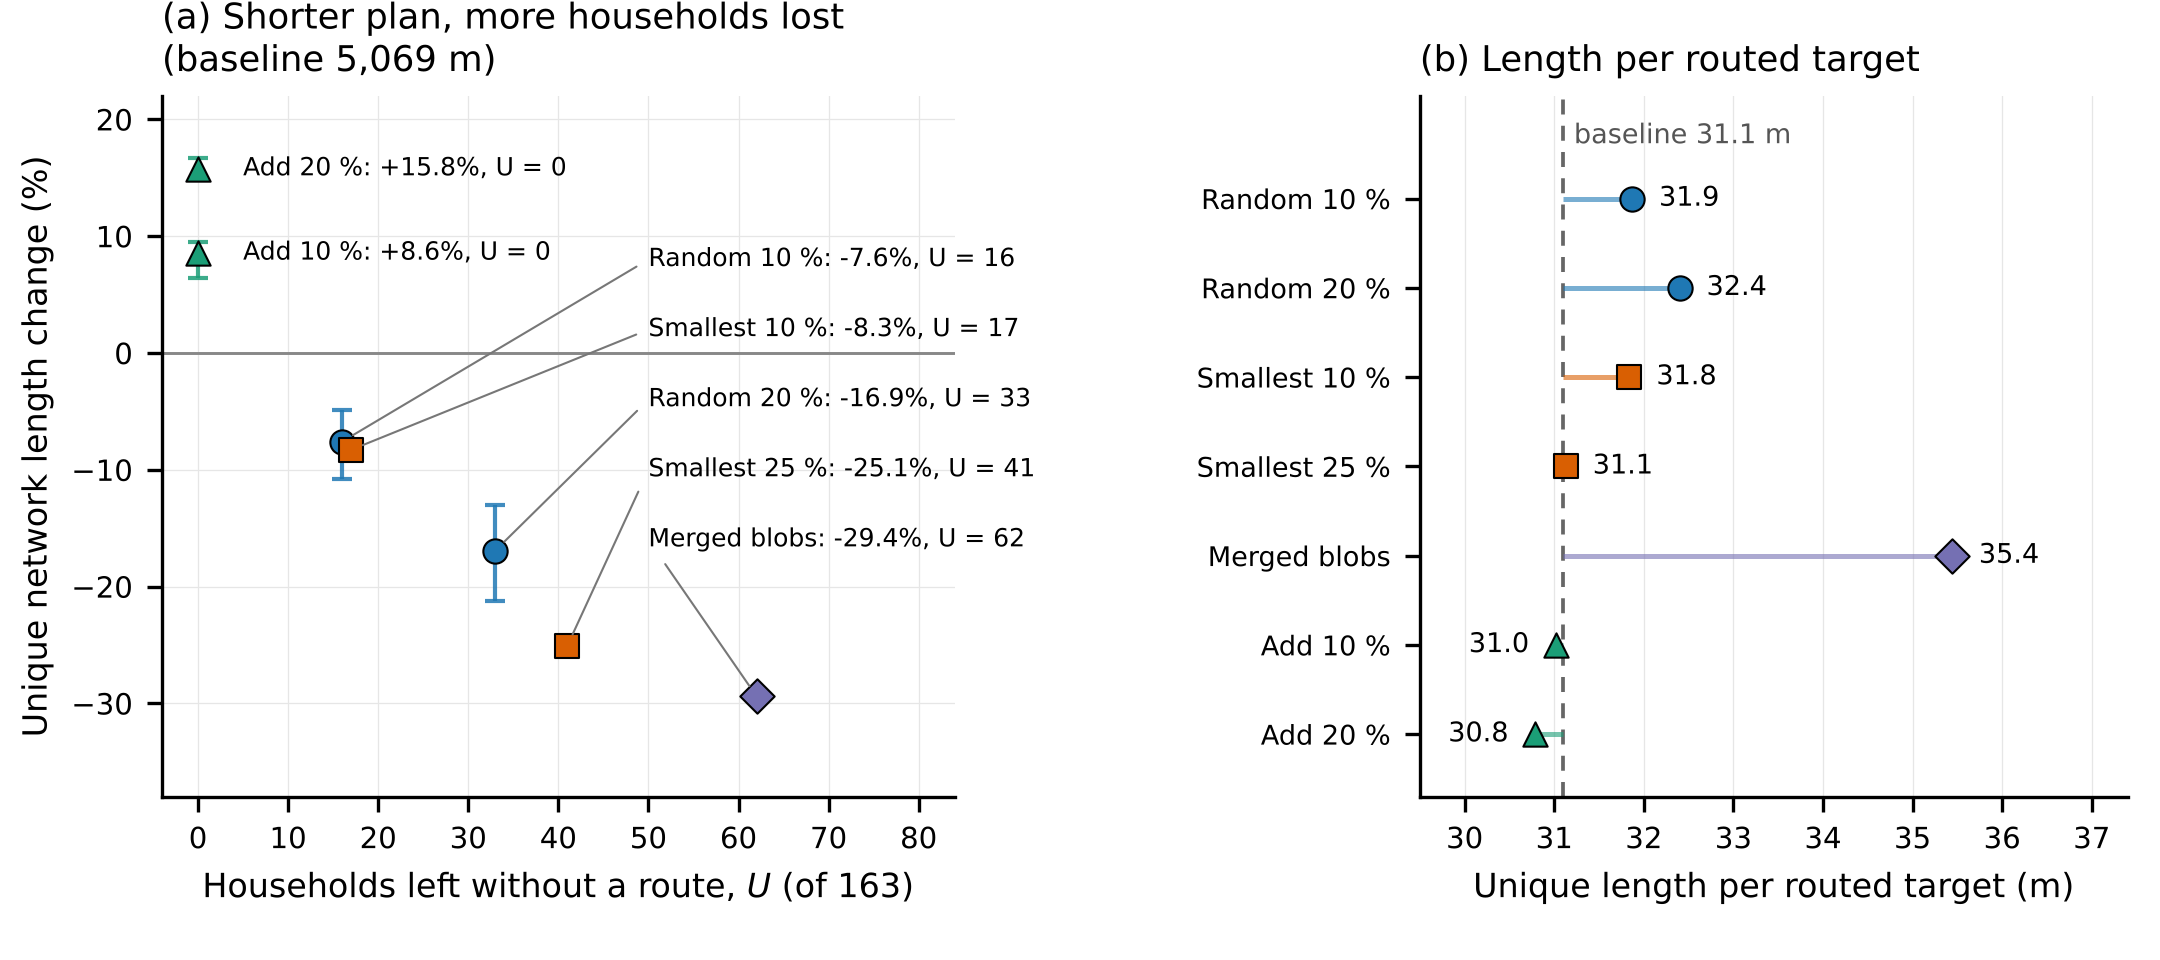
\includegraphics[width=\textwidth]{figures/fig4_omission.png}
\caption{Omission sensitivity, redrawn from the recorded results table (163 baseline targets, 5{,}069~m; random scenarios are five draws with min--max error bars). (a)~Change in unique length against households left without a route: every omission shortens the plan while losing households, whereas additions lengthen it. (b)~Unique length per routed target.}
\label{fig:omission}
\end{figure}

\section{Discussion}
\subsection{Why pixel metrics are not enough for infrastructure use}
The segmentation metric is area-weighted over classes, whereas the planner counts instances. A detector that misses the smallest quarter of buildings by count can lose only a small share of building pixels yet removes a quarter of the households from the plan (table~\ref{tab:omission}); a detector that merges adjacent roofs can score a high pixel IoU yet, as the merged-blob scenario shows, removes 38.0\% of the targets in one stroke. We therefore recommend that detection studies intended for infrastructure use report instance-level recall stratified by footprint size and merge status, and the number of households a downstream plan would leave unserved, alongside mIoU and Dice. The Building-class recall on the source domain (80.6\%) means roughly one building pixel in five is missed, which is the pixel-level counterpart of the omission scenarios, but the village-level false-negative rate is unknown.

\subsection{Land take and environmental implications}
Shared corridors reduce the length of new road for the same set of households. As an illustration, not a design value, assuming a 5~m formation width (an assumption of this study; the project holds no road-width data), the 1{,}684~m saved against independent house-by-house routes corresponds to about 0.84~ha less land take, 2.53~ha for the shared network against 3.38~ha for the unique independent network. The footprint penalty moves the other way: keeping routes out of dwellings costs length, and the buffered variant adds 1.1--1.2~km of corridor, roughly 0.6~ha at the same width, for 19 rather than 28 routes crossing a footprint. Because the 7.1~m buffer and the penalty are modelling choices, a planner needs the length--exposure curve (figure~\ref{fig:routing}b), not one number. The same logic applies to land cover: the cost surface penalises resistant land-cover classes, but we did not quantify the area of cropland or trees crossed, which would be the natural next step for agricultural land-conservation questions. The omission results add that incomplete inventories bias such land-take estimates downward: an inventory missing 20\% of buildings would suggest 16.9\% less corridor, and hence less land, than the full set requires.

\subsection{Planning implications and limitations}
For PMGSY-style schemes \cite{pmgsy}, three practical points follow. First, building inventories are uncertain planning inputs and a network sized from them should carry a sensitivity band. Second, shared corridors save about a quarter of the unique length and this saving survives omissions, which makes sharing a robust argument even where inventories are poor. Third, local overrides should be used sparingly and reported separately. The plans are not checked against Indian Roads Congress or PMGSY technical specifications (curvature, gradient, width, drainage), which the cost surface does not encode; the only engineering constraint is the 25$^{\circ}$ slope block.

Limitations are as follows. The study covers one village, and the omission scenarios are synthetic, not measured detection errors. The candidate layer has no surveyed reference: there is no manual building mask or field survey, and the LoveDA figures come from the epoch-4 checkpoint with metadata recovered from the training notebook; the checkpoint hash was not logged with the village candidates. The planner is greedy and not globally optimal, and shared-edge credit counts only identical grid edges. Slope derives from a $\sim$30~m DEM of unrecorded source, the road layer is of unverified completeness, imagery dates are not recorded, and the imagery licence for derived products has not been cleared. Seasonal occlusion (canopy, shadow, crop cover) is not modelled, and the footprint penalty is a tunable multiplier rather than a measured resistance. Costs are ordinal.

\section{Conclusions}
A pipeline from satellite imagery to shared access roads connects all 163 houses and five facilities of Damarakunta with 24.9\% less unique corridor than independent routing, and a footprint penalty of 4 halves the number of routes crossing other dwellings for a 7.7\% longer network. Simulated detection errors shorten the plan, drop households from it and leave the relative benefit of sharing unchanged: omitting 20\% of buildings at random understates corridor length by 16.9\% and leaves 33 households unplanned, and omitting merged roofs leaves 38.0\% unserved. Pixel scores would not reveal this. Rural road planning that relies on automatically extracted buildings should therefore report instance-level recall and unserved households, and treat corridor length and land take as ranges. Validating the segmenter and the omission patterns on a hand-labelled subset, and quantifying the land cover crossed, are the next steps.

\ack
The author acknowledges the Telangana State Remote Sensing Application Centre (TGRAC) for the boundary, road and facility layers, and the providers of the open datasets used (ESA WorldCover, Google Open Buildings, LoveDA).
% TODO (author): add supervisor / institutional acknowledgements.

\section*{Funding}
% TODO (author): state funding sources, or confirm that none was received.
[Funding statement to be completed by the author.]

\section*{Data availability statement}
The derived result tables (routing, omission and sensitivity runs), the building-candidate layer, the TGRAC-derived planning layers used here, the planner and analysis scripts, and the figure-generation script are available in the project repository (\url{https://github.com/Archana519/Telangana-Rural-Project}, folder \path{DELIVERABLES_DAMARAKUNTA_STAGE_B} and \path{paper/erl}). The LoveDA epoch-4 confusion matrix is in the supplementary file \path{paper/erl/supplementary/loveda_epoch4_confusion_matrix.csv}. The 0.6~m imagery mosaic is third-party data (Esri) and is not redistributed, because the licence for derived products has not been cleared; the geometry of the planned routes of the primary run is not archived in the repository. ESA WorldCover and Google Open Buildings are openly available from their providers. A permanent archive with a DOI will be deposited on acceptance. % TODO (author): create the Zenodo deposit and insert its DOI.

\section*{Conflict of interest}
The author declares no competing interests. % TODO (author): confirm.

\bibliographystyle{\ERLbst}
\bibliography{references}

\end{document}
